%% Sample-Paper.tex
%% V1.0
%% Developed for Authors to create their manuscript.
%%
%% This file uses the coding defined in the LaTex template ICED-Paper.cls

\documentclass{ICED-Paper}%%%%where ICED-Paper is the template name

%The authors can define any packages after the \documentclass{ICED-Paper} command.

%\usepackage{algorithmic} for describing algorithms
%\usepackage{subfig} for getting the subfigures e.g., "Figure 1a and 1b" etc.

%The author can find the documentation of the above style file and any additional
%supporting files if required from "http://www.ctan.org"

% *** Do not adjust length that controls the trim size and margins ***

\begin{document}

%The title of the paper, names of authors, affiliations of authors, abstract
%and keywords for the paper \textbf{will be produced automatically} from the
%ConfTool conference management system, based on the data that you enter in
%the ConfTool. So, don't include those details in this document.
\iffalse
What about figure \ref{fig1}?

\begin{figure}
\centering{
\includegraphics{Fig1.eps}}% Replace "fig1" with appropriate figure file name
\caption{Figure caption here\label{fig1}}
\end{figure}

Text here.

\begin{table}
\processtable{Table title here\label{tab1}}
{\tabcolsep=2pc\begin{tabular}{|l|c|}%Number of columns has to be defined here
\hline
Table text here & Table text here\\%Table body
\hline
Table text here & Table text here\\%Table body
\hline
\end{tabular}}{Table footnote here}
\end{table}
\fi

\section{Introduction}
\iffalse
    here we have to define what is the current state of understanding this phenomenon in the context of design studies and research,
    Open Source is an example of peer production in the sense that there is distributed and not centrally controled, peer to peer basis
    p2p collaborative model, management of the collaboration process,
\fi

\bigskip

\subsection{The emergence of Open Source Design}
\iffalse
In the last three decades the progressive and massive adoption of computers and the internet have opened new possibilities to collaborate in unprecendented ways.Perhaps the most intriguing and solid example of this socio-technical phenomenon is the rise of the FREE/Software movement and the open source model in the software industry.
\fi

It is well known that Free Open Source Software(FOSS) rejects the distribution of software under copyright proprietary licenses and encourages the four basic user freedoms as part of its core philosophy\cite{Freedoms}: \emph{the freedom to use, study, improve and distribute the source code}. This profound paradigm shift has challenged traditional business models and classical economics assumptions that promote intellectual property as a competitive advantage \cite{Para_shift}. Further more it has shown in practice a very different approach to product development in contrast with traditional design and engineering methodologies \cite{HowItWorks}, \cite{bazaar}.
\bigskip

Over the last three decades there has been an increasing commercial adoption of free open source software (FOSS) \cite{Adoption}, being Linux OS perhaps the most emblematic case. Some of most widely used distributions of Linux includes Android(mobilephones),Ubuntu, Debian, Fedora among other thousands of distributions\cite{}. Redhat is perhaps the most known Linux based company,  The Limux project is an example FOSS Linux in public sector \cite{Limux}, which consisted in the migration of local government software from proprietary software to FOSS.There is an extensive body of empirical research that analyzes the open source software phenomenon from different angles ranging from innovation studies\cite{HowItWorks}, to organizational \cite{ActivityTheoryOpenSource} and economic studies \cite{Economics}. Von Hippel has researched open source projects revealing a different model of work that is more collaborative, open and intensively led by users \cite{HowItWorks},\cite{hippel_4},\cite{hippel_2}.
\bigskip

Similarly there has been an increasing adoption of the FOSS philosophy and practices in the hardware domain labeled as Free Open Source Hardware (FOSH)\cite{FH}, \cite{what_OH} (see Rubows technical report on FOSH \cite{Rubow} for an overview of open hardware projects until 2008). Arduino microcontrollers and RepRap 3D printers are perhaps the most prominent products in open hardware, with not only considerable adoption, but also with considerable commercial success. Adafruits and Sparkfun are two well known vendors of open hardware projects. In the case of Adafruits it is quite well known that its founder Limor Fried, also collaborates intensively within the Open Hardware Communities \cite{Million_Dollar}. Some scholars have already shed light on the similarities and differences of FOSS and FOSH, as well as critical success factors to transfer and adopt open source in the context of tangible products, \cite{OSTangible}, \cite{OSTangibleGoods}, as well as in the context of the manufacturing domain \cite{digitalCommons}. These body of research sheds light on the similarities of FOSS and FOSH but also emphasize that the experience is not directly transferable without adaptations and domain related considerations in the context of tangible goods. There is still an ongoing debate on the potentials and limitations of transfering open source software practices and tools in the context of tangible products.
\bigskip

\subsection{Research goals}

\emph{Without a substantive understanding of the historically changing character of the work done in a given organization, theories of design are likely to remain too general and abstract to capture the past vestiges and the emerging possibilities of design}\cite{ExpansiveDesign}

\bigskip

Design Theory and Methodology should study with carefull attention how open source works and evolves overtime. These implies analyzing the specific theories and methodologies used in open source projects, as well as those practices transfered to the domain of tangible products. Moreover this should lead to a more detailed description of how open source related theories, methodologies and practices.
\bigskip

The aim of this work is shed some light on key features of the open source approach to product development in software and hardware. To speficy more this endeavor we ask the following questions:
\bigskip

\begin{itemize}
  \item What characterizes design related activities in the context FOSS and FOSH?
  \item Is there a particular structure or pattern in open source design that charaterizes open source projects?
\end{itemize}


\section{Methodology}
This section describres the theoretical background we have used to analyzed six open source projects (three software and three hardware projects).We use the Activity Theory framework to study open source projects, with a specific focus on the peer-to-peer aspects of the process. Activity Theory studies human behavior in a holistic fashion, and rejects the notion of isolated individual action as a unit of analysis. The main reason to choose this framework is its convenience to study and describe human action and practices in a socio-technical system.

We firstly introduce the notion of commons based peer production, followed by a brief description of what  Activity Theory is and how we have used it to study the open source projects selected, with a special focus on the peer production dimension.

\subsection{Understanding open source projects as peer production systems}
\emph{In a sense, hardware is becoming much more like software, up to the point where you actually fabricate an object,"von Hippel says. "That's why you're starting to see open source techniques in hardware. Design is largely going to shift out from manufacturers to the communities}\cite{OH_works?}
\bigskip

The ammount of participants in open source projects can go from ten to thousands of persons, depending on the project/community. Most well known projects work in a very descentralized and open way and do not fit with traditional industrial paradigms. It has been found that in open source software projects, users lead directly the product development process in contrast with traditional roles in the software industries\cite{HowItWorks}.
\bigskip

Authors like Eric Von Hippel \cite{hippel_2}, Benkler \cite{Benkler} and Bauwens \cite{p2pEconomy} study open source projects considering a community centered approach. In these context open source is understood as a socio-technical phenomenon consisting of key relations that includes cultural, ethical, economic, technological and societal aspects, as part ot their unit of analysis. These group of authors stress the notion of peer to peer based collaboration as a key element to understand this phenomenon. While Von Hippel calls it \emph{free user to user assistance}, Bauwens calls it peer to peer and Benkler refers to it as Commons Based Peer Production(CBPP). These authors emphasize a holistic approach to this phenomenon. They give particular attention to the conditions(social, economic, technological,cultural, etc) in which these models work, succeed and evolve.
\bigskip

For the purposes of this work, and based on the research done by these authors, we will adopt the \emph{commons based peer production(CBPP)} term. We also adopt the a general characterization of CBPP Activity Systems according to Bawuens \cite{p2pEconomy}:

\emph{P2P specifically designates those processes that aim to increase the most widespread participation by equipotential participants. We will define these terms when we examine the characteristics of P2P processes, but here are the most general and important characteristics.
P2P processes:}

\begin{itemize}
  \item \emph{produce use-value through the free cooperation of producers who have access to distributed capital: this is the P2P production mode, a 'third mode of production' different from for-profit or public production by state-owned enterprises. Its product is not exchange value for market, but use-value for a community of users.}
  \item \emph{are governed by the community of producers themselves, and not by market allocation or corporate hierarchy: this is the P2P governance mode, or 'third mode of governance.'}
  \item \emph{make use-value freely accessible on a universal basis, through new common property regimes. This is its distribution or 'peer property mode': a 'third mode of ownership,'different from private property or public (state) property.}
\end{itemize}

\subsubsection{Using Activity Theory to understand CBPP in open source projects}
For a more in depth understanding of AT see \emph{Activity Theory in a Nutshell} \cite{ATnuthsell}. Introducing AT and its full potential of design research and practice goes beyond the scope of this work. The following description gives only a very simplified and summarized introduction to what is AT, and how we used it to study the projects.

\begin{figure}
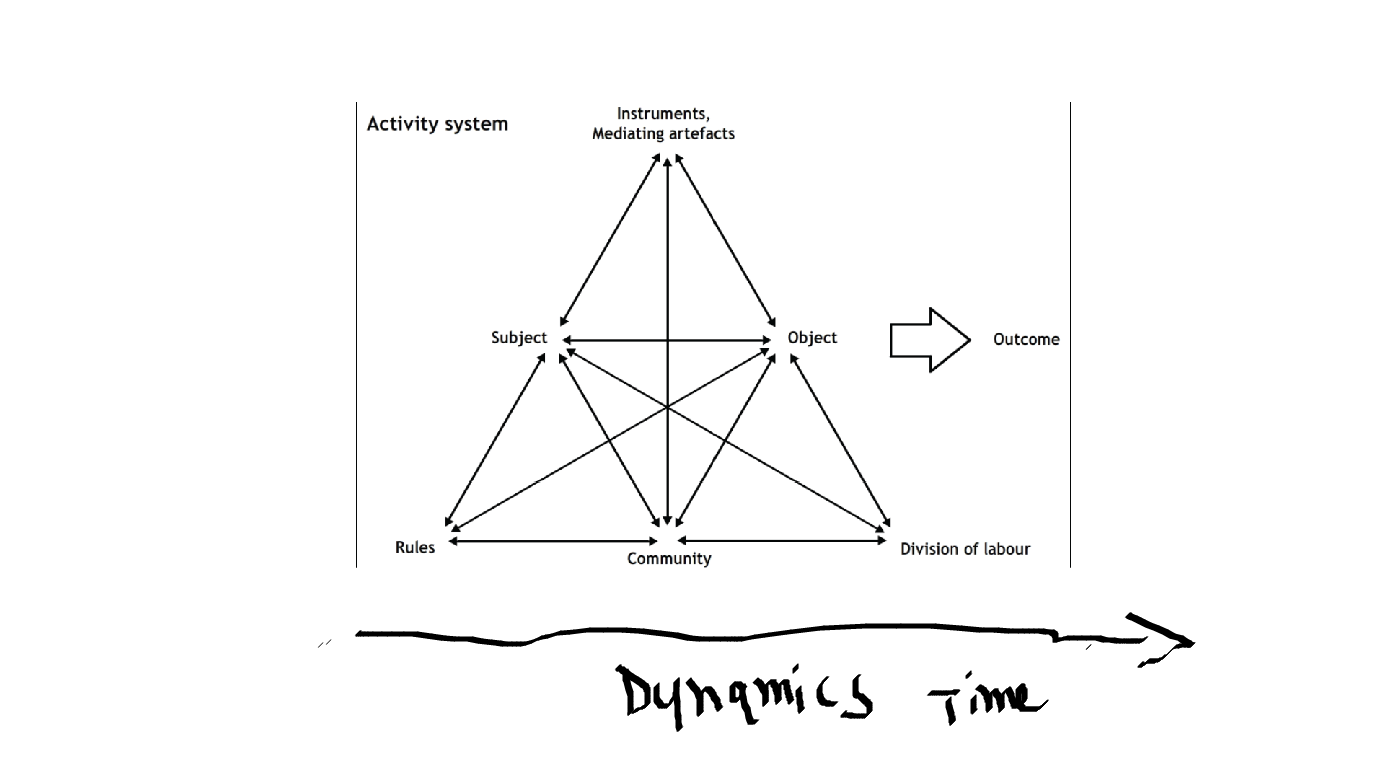
\includegraphics[width=\linewidth,height=\textheight,keepaspectratio]{Activity System.png}
\caption{Figure caption here\label{fig1}}
\end{figure}

\bigskip
\textbf{Object-orientedness}– When a people design and develop, they always design/develop something (an Operating System, a 3D printer). \emp{The world pr
ovides resistance and affordances to our attempts to reach the objects of our activities; through resistance and affordances, objects constrain and direct what we do. We also develop internal, subjective counterparts of the objects, which may be no less effective in constraining and directing our activities than the resistance and affordances of the world. Therefore,objects can be considered as both external and internal}
\bigskip

\textbf{Mediation}-First, tools shape the way human beings interact with reality. And, according to the principle of internalization–externalization, the shaping of external activities eventually results in the shaping of internal ones.econd,
tools usually reflect the experience of other people who tried to solve similar problems earlier and invented or modified the tool to make it more efficient and effective. Their experience is accumulated in the structural properties of tools, such as their shape or material, as well as in the knowledge of how the tool should be used. Tools are created and transformed during the development of the activity itself and carry with them a particular culture—the historical evidence of their development. So the use of tools is an accumulation and transmission of social knowledge. It influences the nature of external behavior and also the mental functioning of individuals.


\textbf{Subject or internalization} – actors engaged in the activities; the traditional notion of mental processes
**Community or externalization** – social context; all actors involved in the activity system
**Tools or tool mediation** – the artifacts (or concepts) used by actors in the system. Tools influence actor-structure interactions, they change with accumulating experience. In addition to physical shape, the knowledge also evolves. Tools are influenced by culture, and their use is a way for the accumulation and transmission of social knowledge. Tools influence both the agents and the structure.
**Division of labor** – social strata, hierarchical structure of activity, the division of activities among actors in the system
**Rules** – conventions, guidelines and rules regulating activities in the system


\subsection{Open source projects for hardware and software}

\subsection{Research questions}
This works a step forward towards understanding


\subsubsection{Understanding design activity in the context of peer production}

\section{Methodology}
This work attempts to capture significant aspects of peer to peer dynamics in the context of open source projects. To map these contexts we use Activity Theory framework[REFERENCE]. This framework allowed us to capture patterns of behavior and collaborative dynamics similarities and differences, beyond the specificities of what tools or systems are used, how tools reflect intagible aspects of socio-technical systems like values, motivations, community rules as well as roles within collaborative dynamics.
\subsection{Specifying free based peer production}
- [ ] Peer to peer happens everywhere, but open collaborative peer to peer means that also unknown peers, in many cases directed unrelated with other peers geographically, ....
\subsection{An overview of  the Activity Theory framework}
This research uses the expanded Activity Theory framework developed by Engestrom [REFERENCE]. This framework provides a consistent model to analyze collective processes like product design and development as part of a social context. This approach considers tools and procedures as part of a broader set of human interactions.
\subsection{Experimental design}
\iffalse
    here I explain the case selected, the rationale behind this selection, as well as the materials used, but also specific questions to answer the general questions,
\fi
We describe at a Meso level these projects as activity  systems that evolve overtime, and how their community composition, activity objects, as well as roles, rules, and artifacts reflect such evolution. Furthermore we attempt to describe how the outcomes of the activity system develop, along with the activity structure.

The two sets of cases (three for software, and three for hardware) are analyzed independently with respect to their own differences and similarities considering the different components of the Activity System model.
- What is the main object of the activity
- What is the main outcome(s) or product(s) of such activity
- What rules and tools they use to organize their collaboration
- What interesting aspects stand out in the case with regard to the outcomes, motivations, expectations as well as the collaboration process.



- Case study of diverse open source software and hardware projects with different characteristics:
We selected projects that present basic similarities with regard to basic freedoms mentioned in the previous section:
- For both sets of cases there is considerable difference in scope, product architecture, documentation, participation,tools but also in age. These set allows us to verify how time reflects in project maturity, adoption of modern practices, but also consistencies regardless of these differences.
- For the software projects there is a main similarity: they all use git based peer review tools.

### Materials
- Interviews and talks from founders of free software and open source movement.
- Forums of different projects like RepRap.
- Project and product documentation
- The Authors familiarity with certain open source projects.
- The availability of data like discussions, documentation, and resources to pursue this study.

### Procedure

Later on key differences and similarities between the two sets are described and discussed considering also the same questions points.

\section{Findings}

In this section we expose some prominent characteristics of the peer to peer interactions using the Activity Theory framework. We study at a very general level how peer to peer relations and interactions are reflected on the artifacts, object, subject, community, rules and division of labor components of the Activity System model.

\subsection{Essential artifacts in free based peer production activities}
From an Activity Theory stand point we can identify many artifacts within open source projects based on the different processes that take place. Mapping out all these artifacts is beyond the scope of this work. Nevertheless there are specific artifacts that are essential to enable an open and horizontal peer to peer collaborative process, or what we have been calling peer production artifacts:
- **Foundational artifacts**. These kind of artifacts describe in broader terms the main rules of the game for open source projects. Among these artifacts we can find perhaps the most important which is the **license** under which the content(source) is released (open) to the public.**Licenses** describe in legal terms what can and cannot be done with the source code ranging from ethical issues to commercial and distribution issues. They also often describe how to give credit to authors, and properly
release new improvements, but also distribute the content and more. It is interesting to notice that since the FREE Software licenses were created, every open source project has adopted or created similar licenses to distribute and share code, but also visual images as well as CAD files. There are other artifacts the specify how to contribute to the project often called *contributing guidelines*, but also the code of conduct, and instructions on how to participate.
- **Peer content production artifacts** There are variations in the way content creation takes place, but ultimately it requires of a web service, where other peers can access and modify the content created collaboratively. These ranges from dedicated git based services like github, or gitlab (Arduino, ), but also wikis.
- **Peer review artifacts** Like peer content production, peer review relates to a more operational level within the activity system. In the case of software, version control of the code is essential. This can be implemented also in different ways, but the standard and widely used system for version control at the moment in the software industry is git, for several reasons that go beyond our scope. Other tools for peer review such as from mailing lists, forums, and chats were found in both software and hardware cases.

\subsection{The role of users within free based peer production}
\subsubsection{Community based projects led by lead users}

Linus Torvalds, the creator of the Linux kernel, on an interview reveals:
> Every single project I haved worked on was for something I needed.

**We have found in our study that all the open source projects have been developed by lead users that have had some level of dissatisfaction with previous solutions** Lead users according to...

All these projects have started because at a certain point users with particular needs and problems, haven't found or have access to the solution they have been looking for to their problems. Moreover these *lead users* have had the capacities to build a new product, and enabled eventually that other users participate in developing, and improving the open source product in new directions.

For instance Linus Torvalds developed the Linux Kernel partly because he needed, partly because he enjoyed programming, he says that he never imagined Linux would evolve into what it is today. Richard Stallman the father of the FREE/Software movement and the GNU/Linux Project, refused to accept that computer scientists, programmers and users in general were not able to do study the source code.
Josef Prusa, a main contributor in the RepRap community explains in an interview:
>  originally got into 3D printing because I was into music, and I started to build my own MIDI controllers. I needed all sorts of little knobs and faders. So that’s how I found 3D printing. I started to build one myself, but it took so much time and so many parts that I eventually started to make it simpler. I started to improve it and give back, and so that’s how the Prusa Simplified Mendel came to the world.

**Open Source Ecology** was also motivated by the difficulties and circumstances that Marcin Jakubowski experienced after starting a farm:
> I bought a tractor then it broke, I paid to get it repaired, then it broke again....I realized that the truly appropriate, low-cost tools that I needed to start a sustainable farm....just didn't exist.

In the case of Git and Gitlab the original motivation was again to solve problems meeting specific requirements. Git started as a tool for version control on the Linux project. Version control is an essential artifact in the context of software.
>...we were in this bad spot where we had thousands of people
who wanted to participate, but in many ways, I was the kind of break point,where I could not scale to the point where I could work
with thousands of people. So Git is my second big project which was only created for me to maintain my first big project.(Linux)

Similarly Gitlab was started based on a need to collaborate on software development teams by a software developed. In the case of Arduino the main motivation was to create simple and low cost tools for creating digital projects by non-engineers in the an academic context. Before launching the project, the main users teachers and students, had difficulties because of not having a low cost solutions to teach electronics. Before Arduino, it was very expensive for students to work with microcontrollers during their studies.


\subsubsection{Community composition}

\subsection{The continuous expansion of activity objects in free based peer production communities}

\subsubsection{Integrated product extension}

\subsubsection{Product derivatives and variations}

\section{discussion}
\subsection{Domain specificities of software and hardware}

\subsection{Implications for design research and methodologies}

\subsection{Recommendations for further studies}

\section*{References}

\bibliographystyle{unsrtnat}


  %Introduction
  \bibitem{ExpansiveDesign}Engeström, Y., 2006. Activity theory and expansive design. Theories and practice of interaction design, pp.3-23.
  \bigskip

  \bibitem{Freedoms} What is free software?, GNU, accessed 19 November 2017,
  <https://www.gnu.org/philosophy/free-sw.en.html>
  \bigskip

  \bibitem{Para_shift}Maher, M., 1999. Open source software: The success of an alternative intellectual property incentive paradigm. Fordham Intell. Prop. Media & Ent. LJ, 10, p.619.
  \bigskip

  \bibitem{HowItWorks}Lakhani, K.R. and Von Hippel, E., 2004. How open source software works:“free” user-to-user assistance. In Produktentwicklung mit virtuellen Communities (pp. 303-339). Gabler Verlag.
  \bigskip

  \bibitem{bazaar}  Demil, B. and Lecocq, X. (2006) ‘Neither Market nor Hierarchy nor Network: The Emergence of Bazaar Governance’, Organization Studies, 27(10), pp. 1447–1466. doi: 10.1177/0170840606067250.
  \bigskip

  \bibitem{Adoption}Glynn, E., Fitzgerald, B. and Exton, C., 2005, November. Commercial adoption of open source software: an empirical study. In 2005 International Symposium on Empirical Software Engineering, 2005. (p. 10). IEEE.
  \bigskip

  \bibitem{Limux} Free software in government: Munich and LiMux 2017, Free Software Foundation, accessed 19 November 2017, <https://www.fsf.org/bulletin/2017/fall/free-software-in-government-munich-and-limux>
  \bigskip

  \bibitem{ActivityTheoryOpenSource}Hemetsberger, A. and Reinhardt, C., 2009. Collective development in open-source communities: An activity theoretical perspective on successful online collaboration. Organization studies, 30(9), pp.987-1008.
  \bigskip

  \bibitem{Economics}Lerner, J. and Tirole, J., 2005. The economics of technology sharing: Open source and beyond. Journal of Economic Perspectives, 19(2), pp.99-120.
  \bigskip

  \bibitem{hippel_4}Baldwin, C. and Von Hippel, E., 2011. Modeling a paradigm shift: From producer innovation to user and open collaborative innovation. Organization Science, 22(6), pp.1399-1417.
  \bigskip

  %cited
  \bibitem{hippel_2}Von Hippel, Eric. "Democratizing innovation: The evolving phenomenon of user innovation." Journal für Betriebswirtschaft 55, no. 1 (2005): 63-78.
  \bigskip

  \bibitem{FH}Free Hardware and Free Hardware Designs 2015, Richard Stallman, accessed 19 November 2018, <https://www.gnu.org/philosophy/free-hardware-designs.en.html>
  \bigskip

  \bibitem{Rubow}Rubow, E., 2008. Open source hardware. Technical report.
  \bigskip

  \bibitem{what_OH} What is open hardware?,  opensource.com, accessed 19 November 2018,<https://opensource.com/resources/what-open-hardware>
  \bigskip

  \bibitem{Million_Dollar}Torrone, P. and Fried, L., 2010. Million Dollar Baby. Businesses Designing and Selling Open Source Hardware, Making Millions. Talk at the O'Reilly foo camp east, 1.
  \bigskip

  \bibitem{OSTangible}Raasch, C., Herstatt, C. and Balka, K., 2009. On the open design of tangible goods. R&d Management, 39(4), pp.382-393.
  \bigskip

  \bibitem{OSTangibleGoods}Balka, K., Raasch, C. and Herstatt, C., 2009, April. Open source beyond software: An empirical investigation of the open design phenomenon. In R&D Management Conference (pp. 14-16).
  \bigskip

  \bibitem{digitalCommons}Kostakis, Vasilis, Kostas Latoufis, Minas Liarokapis, and Michel Bauwens. "The convergence of digital commons with local manufacturing from a degrowth perspective: two illustrative cases." Journal of Cleaner Production (2016).
  \bigskip

  \bibitem{Benkler}Benkler, Yochai. "Peer production and cooperation." Handbook on the Economics of the Internet 91 (2016).
  \bigskip

  \bibitem{p2pEconomy}Bauwens, M., 2005. The political economy of peer production. CTheory, pp.12-1.


\end{thebibliography}
\section*{Acknowledgments}

Acknowledgments text here.

\appendix

\section*{Appendix}

Appendix text here.

\end{document}
